\documentclass{article}

\usepackage{amsmath}
\usepackage{amssymb}
\usepackage{graphicx}
\usepackage{array}
\usepackage{url}

\DeclareMathOperator*{\argmax}{arg\,max}

\newcolumntype{L}[1]{>{\raggedright\let\newline\\\arraybackslash\hspace{0pt}}m{#1}}

\begin{document}

\title{Assignment 1}
\author{Cameron Salisbury}

\maketitle

\section{Introduction}

In this report I will describe my implementation of the Spherical K-Means algorithm which extracts features from images based on the description in the paper~\cite{paper}. This implementation has been written in Java using the WEKA API~\cite{weka} and a template that implemented part of the algorithm already. This report will also discuss some results obtained when using this algorithm as a preprocessor for various classification problems.

\section{Method}

This algorithm is implemented as a filter using the WEKA API~\cite{weka} along with the MTJ library~\cite{matrix_lib} for the matrix calculations. The algorithm has two main parts, initialization, which uses the training data to create a dictionary that can then be used in the second part, feature extraction, which extracted features (i.e. an array of numbers) from an image which can then be used for some other purpose.

\subsection{Initialization}

The initialization part of the algorithm is described in the paper~\cite{paper} in section 2 and is  split into two subsections. The part of the algorithm described in section 2.1 was already implemented in the template that was provided and extracted a user specified number of random square patches of size $p\textrm{-by-}p$, where $p$ is a user specified size value. The red, green and blue values of the of the pixels in the extracted patches were then used to form vectors $x^{(i)} \in \mathbb{R}^n$, where $n$ is the number of values extracted from the patch, which were normalised as per the equation described in the paper with $\epsilon_{\mathrm{norm}}=10$:
\[
x^{(i)} := \frac{x^{(i)} - \mathrm{mean} \left( x^{(i)} \right) }{\sqrt{\mathrm{var} \left( x^{(i)} + 10 \right) }}, \forall i
\]
These vectors where then used to construct the matrix $X \in \mathbb{R}^{n \times m}$, where $m$ is the number of patches, and that data is then whitened as per the equation described in the paper with $\epsilon_{\mathrm{zca}}=0.1$:
\[
[V,D] := \mathrm{eig} \left( \mathrm{cov} \left( X \right) \right) ; \textrm{ // So } VDV^{\mathrm{T}} = \mathrm{cov} \left( X \right)
\]\[
X := V \left( D + 0.1 \boldsymbol{I} \right) ^{-1/2} V^{\mathrm{T}} X
\]
By using these two processes to pre-process the data we will get better results from the K-means algorithm.

\paragraph*{}

The next part of the algorithm, which I implemented, is described in section 2.2 of the paper generates the centroids which will be used to extract features from the images. To begin with a matrix $\mathcal{D} \in \mathbb{R}^{n \times k}$, where $k$ is the number of centroids to use specified by the user, is filled with random values sampled from a normal distribution and then each column in the $\mathcal{D}$ is normalised to unit length. This matrix $\mathcal{D}$ is our dictionary of centroids, where each column is one of our centroids on the unit sphere. We now need to optimise this dictionary. This starts by calculating the matrix $S \in \mathbb{R}^{k \times m}$:
\[
S := \mathcal{D}^{\mathrm{T}} X
\]
giving us a matrix where each column represents one of the patches in $X$ and each value in that column is the dot product between the patch and centroid. As the absolute value of a dot product is minimised when two vectors are orthogonal and maximised when they are collinear, we can think of these values are representing how closely the patch matches the centroid. So we then modify $S$ to keep only the largest value absolute in each column:
\[
s^{(i)}_{j} := 
\begin{cases}
s^{(i)}_j & \textrm{if } j = \argmax\limits_{l} \left| s^{(i)}_l \right| \\
0 & \textrm{otherwise}
\end{cases}
, \forall i,j
\]
giving us a matrix that assigns each patch to the centroid it matches most closely.

\paragraph*{}

In the paper it suggests iterating a fixed number of time, saying 10 should be enough, but my implementation uses a different approach and calculates the sum of squared error:
\[
\mathrm{SSE} = \left\lVert \mathcal{D}S - X \right\rVert_{\mathrm{F}}^{2}
\]
and checks if the sum of squared errors this iteration, $\mathrm{SSE_{new}}$, has changed enough since the last iteration, $\mathrm{SSE_{old}}$, by checking if:
\[
\frac{\mathrm{SSE_{old}} - \mathrm{SSE_{new}}}{\mathrm{SSE_{old}}} < 10^{-12}
\]
and stops the iteration process if this condition is meet. Because the algorithm converges this condition should eventually be meet, stopping the iteration process, but there is also a hard limit of 200 iterations (although this limit has never been reached on any test data).

\paragraph*{}

The next step is to reinitialize empty centroids which the paper suggests can improve performance. This is done by searching $S$ to find rows with no non-zero values. If a row like this is found, the corresponding column in $\mathcal{D}$ is replaces with a random patch from $X$ and that new column is then normalised. This replaces the empty centroid with a centroid that is guaranteed to be non-empty. It is worth noting as the patches have already been allocated this iteration this new patch will not be optimised this iteration. If on any iteration no empty centroids are found, no future iterations will check for empty centroids so in practice if $k$ is selected well this step should only be performed on at most a couple of iterations.

\paragraph*{}

Finally, the dictionary is optimised as per the equation:
\[
\mathcal{D} := XS^{\mathrm{T}} + \mathcal{D}
\]
and then each column in $\mathcal{D}$ is normalised again. This whole process is repeated again until the previously described escape condition is meet. In the end we end up with centroids like those in Figure~\ref{centroids}, which in theory should represent simple features found in the training images.

\begin{figure}[h]
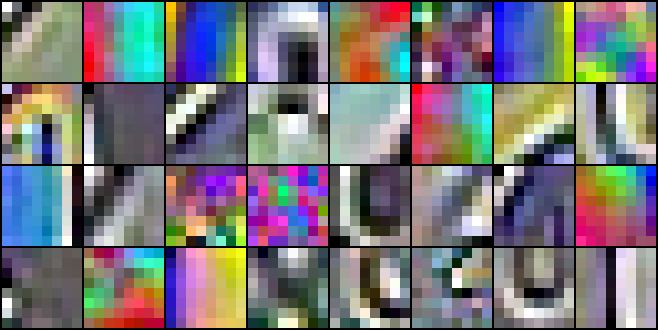
\includegraphics[width=\linewidth]{centroids.png}
\caption{A selection of centroids generated when running the algorithm on the svhn~\cite{svhn} dataset.}
\label{centroids}
\end{figure}

\subsection{Feature Extraction}

The algorithm then proceeds to extract features from images using the dictionary $\mathcal{D}$ as described in by the paper~\cite{paper} in section 4. The algorithm takes one image at a time and extracts patches from that image of size $p\textrm{-by-}p$, starting from the top left and stepping along by some stride specified by the user. The pixel values are then extracted from the patches in same way as before and normalised using the same equation before being set as the columns of the matrix $P \in \mathbb{R}^{n \times w}$, where $w$ is the number of patches extracted from the image. These patches are then compared to the centroids using the calculation:
\[
F := \mathcal{D}^{\mathrm{T}}P
\]
where each column in the matrix $F$ represents a patch from the image and each value in the column is how closely that column matches the specific centroid.

\paragraph*{}

The patches extracted from the image are then grouped into pools of $u\textrm{-by-}u$ patches, where $u$ is some user specified value, to reduce the number of features by $u^2$. The pooling is done by summing the values in $F$ in the same pool and for the same centroid, treating any negative values as 0. All of these pooled values are then put into a final array of features which can then be used by some classification model.

\section{Experimental results}

In Table~\ref{data} you can see the some of the results produced using my K-means algorithm. These were generated using WEKA~\cite{weka} using the command: \\
\texttt{java weka.Run .FilteredClassifier -o -v -t training.arff -T  \\
testing.arff -F .KMeansImageFilter -W .MultiClassClassifier -- \\
-M 3 -W .SGD -- -N -M -F 0 -L 0.0001 -E 100} \\
so the data was first filtered by my K-means algorithm then run through a multi-class classifier using the stochastic gradient descent (SGD) classifier. The results show the K-means filter allows for very accurate classification of the mnist~\cite{mnist} dataset, which consists of grayscale images of hand drawn number, whereas for the more complex fashion-mnist~\cite{fashion} and svhn~\cite{svhn} datasets, which are grayscale images of clothing items and house number from Google Street View respectively, performance is considerably worse, but still ok. For the cifar-10~\cite{cifar} dataset, a dataset of 10 kinds of vehicles and animals, the classification performance is rather poor, so while the K-means filter does appear to work well in some situations, it is limited in terms of the complexity of the datasets it allows for accurate classification of.

\begin{table}[h]
\center
\begin{tabular}{| L{2.1cm} | L{1cm} | L{1cm} | L{1cm} | L{1.8cm} | L{1.8cm} |}
\hline
Dataset & Image Size & Stride Size & Pool Size & Training Data Error Rate & Testing Data Error Rate \\
\hline
mnist         & 24x24 & 4 & 2 & 0.05\%  & 1.63\%  \\
fashion-mnist & 24x24 & 4 & 2 & 3.41\%  & 10.44\% \\
cifar-10      & 32x32 & 4 & 2 & 19.82\% & 35.6\%  \\
svhn          & 32x32 & 4 & 2 & 9.55\%  & 16.50\% \\
\hline
\end{tabular}
\caption{Results when using K-means filter on mnist~\cite{mnist}, fashion-mnist~\cite{fashion}, cifar~\cite{cifar} and svhn~\cite{svhn} datasets.}
\label{data}
\end{table}

\paragraph*{}

In Table~\ref{compare} we can see a comparison between the K-means filter and some filters in the ImageFilter package~\cite{imagefilter} for WEKA, specifically the pyramid histogram of oriented gradients (PHOG) filter and edge histogram filter. These filters were used as a direct replacement for the K-means filter to get these results and were the two best preforming filters from the ImageFilter package. These two filters result in significantly worse classifications on these datasets than the K-means filter, with error rates ranging from 1.6 to 5.9 times higher, so compared to algorithms with similar purposes the K-means algorithm does appear to be a strong alternative.

\begin{table}[h]
\center
\begin{tabular}{| L{2.1cm} | L{2.5cm} | L{2.5cm} | L{2.5cm} |}
\hline
Dataset & K-means Error Rate & PHOG Error Rate & Edge Histogram Error Rate \\
\hline
mnist         & 1.63\%  & 5.12\%  & 9.64\% \\
fashion-mnist & 10.44\% & 19.59\% & 21.87\% \\
cifar-10      & 35.6\%  & 62.34\% & 57.40\% \\
svhn          & 16.50\% & 35.16\% & 30.93\% \\
\hline
\end{tabular}
\caption{Comparison of results between K-mean and filters from the ImageFilter package.}
\label{compare}
\end{table}


\section{Conclusions}

This report explains my implementation of the Spherical K-means filter algorithm described in the paper~\cite{paper}. The report then showed some results produced when the K-means filter is used in some classification problems and compared those results to the results obtained from using other image filters designed to fulfil a similar purpose. From these results we saw that the K-means filter produced better results than these alternatives and while the K-means filter could be used to classify some datasets well, it did not perform particularly well on more complex datasets.

\bibliographystyle{plain}
\bibliography{report}

\end{document}
